\section{Fallstudie}
\begin{comment}
subsection{Fallstudie Rossi Notes}

Fragestellungen:
Wie kann das 3D Modell eines Gebäudes zu einem für einen Roboterschwarm abarbeitbaren Bauplan umgewandelt werden?
Folgefragen:
Wie werden Gebäude heutzutage modelliert? (Revit, Blender -> IFC BIM)
Wie sieht das Format des 3D Modells aus? (IFC)
Was sind gägnige Praktiken beim Planen eines Bauprojekts? (BIM)
Wie ist der aktuelle Stand der Automatisierung im Bereich Konstruktion? (Related Work)
Welche Projekte bauen schon mit Roboter(schwärmen) Gebäude/Gebilde? (Related Work)
Welche Schwierigkeiten gibt es? (Related Work)
Wie sieht so ein Bauplan aus? (Ludwigs Diss)
Welche Schwierigkeiten gibt es bei der Erstellung so eines Bauplans?  (Ludwigs Diss)

Fallstudie:
Modellieren eines Gebäudes in einem 3D Editor, welches anschließend in einen Bauplan überführt wird.

Suche:
3D Editor.
Speicherformat für 3D Modelle.

Probleme: 
Analaysie des 3D Modells auf für uns notwendige Teile (Wände zb)
Mit einbeziehen sämtlicher Constraints von Robotern und Bauteilen (Form Bewegungseinschränkungen Stapelbarkeit etc).
Für Roboter erstmal nicht überbrückbare Lücken wie Fenster Türen.
Guten/Besten Bauplan generieren (Ludiwgs Diss).

Heterogener Roboterschwarm baut Haus mit Fenstern und Türen (Lücken)
Wie werden arbiträre Bausteine beschrieben, damit damit dann ne Wand gefüllt werden kann. Kann man die Bausteine schneiden und wenn ja wo und welcher Weise?


\begin{figure}
    \centering
    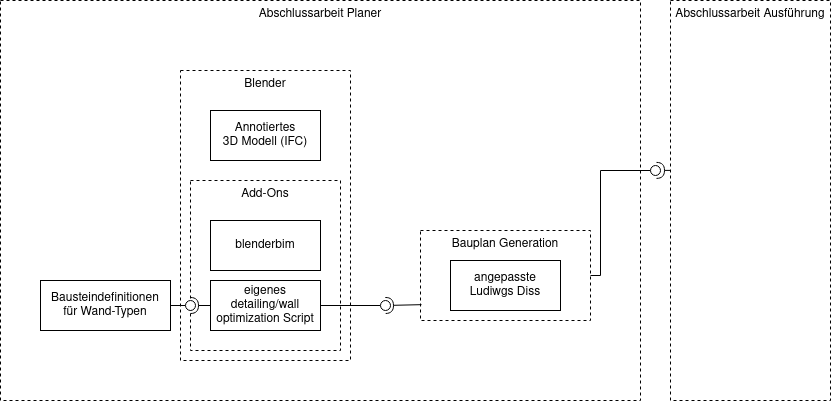
\includegraphics[width=0.9\columnwidth]{fig/structure.drawio.png}
    \caption{Aufbau der Abschlussarbeiten}
    \label{fig:Structure}
\end{figure}

Die Fallstudie unterteilt sich in zwei Teile, die jeweils von einer selbständigen Abschlussarbeit bearbeitet werden.
Der vorliegende erste Teil behinhaltet das Modellieren eines Gebäudes in einem 3D Editor und das anschließende Analysieren und Errechnen eines Bauplans.
Der Bauplan soll im zweiten Teil der Fallstudie von speziell dafür entwickelten Robotern durchgeführt werden, die sich auf den Mauern des Gebäudes selbst bewegen.
Dabei soll das Gebäude Elemente wie Fenster und Türen enthalten, um dem Problem von Lücken innerhalb einer Wand zu begegnen, welche ein Hindernis für die darauf fahrenden Roboter darstellen.
Das Errechnen eines Bauplans ausgehend von einem 3D Modell eines Gebäudes soll für beliebig beschaffene Bausteine möglich sein, welche zuvor definiert werden.
\end{comment}

\subsection{Basis Szenario}
Zu Beginn wird aus dem in Abbildung TODO zu sehenden Modells eines kleinen Hauses ein Bauplan generiert.
Dieses Modell wurde in Blender - erweitert dem IFC Plugin - erstellt und verfügt nur über Wände eines bestimmten Typs, für welchen ein einzelner Bausteintyp definiert wird.
Dieser Bausteintyp definiert einen nicht veränderbaren Quader.
Das beudetet, dass das Bearbeiten der Bausteine, wie etwa das Schneiden eines Ziegelsteins, nicht berücksichtigt wird.
Deshalb wird vorerst vorausgesetzt, dass die Wände des Modells mithilfe dieses Bausteintyps lückenlos "diskretisiert" werden können.
Mit diesem kleinen Szenario wird die Zusammenarbeit aller notwendigen Komponenten ersichtlich und es werden verschiedene Ansätze untersucht, um einige Lösungen für den Bauplan der Wände zu erhalten und zu vergleichen.
Außerdem müssen schon hier Regeln in den Planungsalgorithmus eingeführt werden, die diverse Mauerwerksverbände erzwingen zu können, um damit die Stabilität und gleichmäßige Kraftverteilung in einer Wand zu gewährleisten und sich gleichzeitig möglichst nah an der Realität des Mauerbaus zu bewegen.
Mithilfe der Ergebnisse aus diesem Szenario wird in den Nachfolgenden ein Format zur Definition generischerer Bausteintypen entwickelt und verfeinert.
Zusätzlich wird sowohl die Grundstruktur für die kommenden Szenarios abgeleitet als auch die Eignung von Blender und der IFC-Erweiterung für die Bearbeitung dieser Szenarien überprüft.

\subsection{Konstruktionsplaner für Häuser am Beispiel von LEGO}
Für dieses Szenario sind zwei Wandtypen definiert worden, die mit unterschiedlichen Sets an Bausteintypen errichtet werden sollen.
So gibt es eine breite und eine dünne Wand.
Für breite Wände gilt, dass diese immer 4 Noppen breit und mindestens zwei Noppen lang sein muss.
Das entspricht einem quer gesetzten einzelnen Standardstein.
Für dünne Wände hingegen gilt eine feste Breite von 2 Noppen und eine Mindestlänge von ebenfalls zwei Noppen.
TODO Abbildungen mit den möglichen Bausteinen der beiden Sets.
Das bedeutet, dass es von Nöten ist, dem Nutzer ein Raster für die Bearbeitung diesen Wänden aufzuzwingen, damit der Planungsalgorithmus immer eine lückenlose Lösung finden kann.
Dies ist durch Anpassen der Blender-Bearbeitungsmöglichkeiten für ein mit einem der beiden Wandtypen annotiertes Objek umsetzbar.
Nicht nur die Abmessungen der Wände müssen in ein Raster fallen, auch die Rotation dieser wird in diesem Szenario auf 90\textdegree{} Schritte limitiert. 
Das stellt für dieses Szenario eine vertretbare Enschränkung dar, da es ohnehin dem intuitiven Umgang mit LEGO Steinen und gleichzeitig den Baustil von den meisten einfachen Gebäuden entspricht.
Folglich muss ein Format für die Bausteintypen entwickelt werden, aus welchen all diese Informationen abgeleitet werden können.
Dieses Format muss sowohl innerhalb von Blender verwendet, als auch zur Berechnung innerhalb des Planungsalgorithmus herangezogen werden.
Als zusätzliches Problem werden in dem Szenario Fenster und TÜren, die Lücken in einer Wand darstellen, betrachtet.
Außerdem werden weitere Regeln eingeführt, um den resultierenden Plan näher an das Vorgehen eines realen Baus zu bringen.
So werden beim Errichten von Häusern standardmäßig zuerst die Ecken (der Schnittpunkt zweier Wände) um eine Stufe erhöht, um im Anschluss die geraden Wandabschnitte aufzufüllen.
Damit wird vermieden, dass in den ohnehin schon komplexeren Eckbereichen auch noch zugeschnittene Ziegel notwenig werden.
Stattdessen schneidet man diese erst zurecht, wenn sich dann eher mittig im Wandabschnitt Lücken ergeben, die kleiner sind als die vorhandenen Ziegel.
Zwar wird dies im Fall von Legosteinen nie auftreten, aber es ist übersichtlicher das Problem in dem vorliegenden eingeschränkten Szenario zu beschreiben.

\subsection{Szenario mit veränderbaren Bausteintypen}
Wie können wir die Bausteine veränderbar machen, sprich die Bearbeitungsmöglichkeiten während des Baus (schneiden eines Ziegels) miteinbeziehen in unser Bausteinformat.
Erstmal das schneiden nur parallel zu den ebenen eines rechteckigen ziegelsteins betrachten, denn bei "schrägen" schnitten entstehen neue komplexe Formen..
Wie generiert man daraus dann Baupläne -> riesiges aber cooles Optimierungsproblem!
Vlt geht das richtung constraint programming? Sprich den Bauplan als Lösung für ein beschränktes Problem ansehen.
Total viele Fragen, keine Ahnung wo zu beginnen aber klingt cool

\subsection{Sternchenaufgabe: Szenario mit "runden" Wänden und arbiträren (nicht rechteckige) Bausteinformen / schräge schnitte}
Was machen wir wenn die Wand nicht perfekt mit den vorgegebenen Bausteintypen gebaut werden kann (Beispiel ein runder Turm)
Bausteinverbindungen (wie Mörtel) betrachten und als \textit{Verbindungselement} in das Bausteinformat mit aufnehmen? Wie kann man diesen so einschränken, dass nur physisch machbares ausgrechnet wird.
Was wenn die Bausteine arbiträre Formen haben und nur in sehr komplexen Mustern eine "dichte" Wand ergeben -> tiling Probleme.